%% 
%% Copyright 2007-2025 Elsevier Ltd
%% 
%% This file is part of the 'Elsarticle Bundle'.
%% ---------------------------------------------
%% 
%% It may be distributed under the conditions of the LaTeX Project Public
%% License, either version 1.3 of this license or (at your option) any
%% later version.  The latest version of this license is in
%%    http://www.latex-project.org/lppl.txt
%% and version 1.3 or later is part of all distributions of LaTeX
%% version 1999/12/01 or later.
%% 
%% The list of all files belonging to the 'Elsarticle Bundle' is
%% given in the file `manifest.txt'.
%% 
%% Template article for Elsevier's document class `elsarticle'
%% with harvard style bibliographic references

\documentclass[preprint, 12pt]{elsarticle}

%% Use the options 1p,twocolumn; 3p; 3p,twocolumn; 5p; or 5p,twocolumn
%% for a journal layout:
%% \documentclass[final,1p,times,authoryear]{elsarticle}
%% \documentclass[final,1p,times,twocolumn,authoryear]{elsarticle}
%% \documentclass[final,3p,times,authoryear]{elsarticle}
%% \documentclass[final,3p,times,twocolumn,authoryear]{elsarticle}
%% \documentclass[final,5p,times,authoryear]{elsarticle}
%% \documentclass[final,5p,times,twocolumn,authoryear]{elsarticle}

%% For including figures, graphicx.sty has been loaded in
%% elsarticle.cls. If you prefer to use the old commands
%% please give \usepackage{epsfig}

%% The amssymb package provides various useful mathematical symbols
\usepackage{amssymb}
%% The amsmath package provides various useful equation environments.
\usepackage{amsmath}
%% The amsthm package provides extended theorem environments
%% \usepackage{amsthm}

%% The lineno packages adds line numbers.
\usepackage{lineno}

%% Use this package to add line brakes in URL
\usepackage{xurl}

\graphicspath{ {../Scripts/} }

\journal{Renewable Energy}

\begin{document}

\begin{frontmatter}
	
\newpageafter{author}

\title{Reducing RES Droughts through the integration of wind and solar PV}

\author[Math]{Boris Morin \corref{cor1}}
\ead{boris.morin@ucdconnect.ie}

\author[Math]{Aina Maimó Far}
\ead{aina.maimofar@ucd.ie}

\author[Eng]{Damian Flynn}
\ead{damian.flynn@ucd.ie}

\author[Math]{Conor Sweeney}
\ead{conor.sweeney@ucd.ie}

%% Author affiliation
\affiliation[Math]{organization={School of Mathematics and Statistics, University College Dublin}, %Department and Organization
	addressline={Belfied, Dublin 4}, 
	city={Dublin},
	postcode={D04 V1W8}, 
	country={Ireland}}

\affiliation[Eng]{organization={School of Electrical and Electronic Engineering, University College Dublin}, %Department and Organization
	addressline={Belfied, Dublin 4}, 
	city={Dublin},
	postcode={D04 V1W8}, 
	country={Ireland}}

\cortext[cor1]{Corresponding author}

%% Abstract
\begin{abstract}
Increasing the share of electricity produced from renewable energy sources (RES), combined with RES dependence on weather, poses a critical challenge for energy systems. This study investigates the importance of the balance between wind and solar photovoltaic (PV) capacity on periods of low renewable generation, known as RES droughts. Three different RES datasets are used to estimate the capacity factors for different scenarios of installed capacities for wind and solar PV power. The skill of the RES models is quantified by comparing capacity factor time series to observed hourly data and by assessing their representation of observed RES droughts. The RES models are used to generate a 45-year hourly time series of RES capacity factor, enabling analysis of the frequency, duration and return periods of RES droughts at a climatological scale. Results show the importance of using an accurate, validated RES model for RES drought risk assessment. The addition of solar PV capacity to a wind-dominated system results in a significant reduction in the frequency and duration of RES droughts, while also reducing extremes and seasonal RES drought patterns. These findings underscore the importance of diversification in RES capacity to enhance energy security and resilience.
\end{abstract}

%%Research highlights
\begin{highlights}
\item RES droughts are analysed using 45 years of hourly wind and solar PV generation data

\item RES droughts from C3S-Energy and ERA5-Atlite datasets are compared

\item Adding solar PV to a wind-dominated system reduces RES drought frequency and duration

\item Validated RES datasets are crucial to accurately identify RES drought extremes

\end{highlights}

%% Keywords
\begin{keyword}
RES Drought \sep Wind Power \sep Solar PV Power \sep Renewable Energy Sources \sep Return Periods

\end{keyword}

\end{frontmatter}

%% Add \usepackage{lineno} before \begin{document} and uncomment 
%% following line to enable line numbers
\linenumbers

\section{Introduction}
\label{sec:intro}

The EU aims to generate at least 69\% of its electricity from renewable energy sources (RES) by 2030, up from 41\% in 2022~\citep{eurostat2023share}. While this transition is essential for reducing greenhouse gas emissions, it also highlights the challenge of managing the variability of weather-dependent energy sources such as wind and solar photovoltaic (PV) power. This challenge is amplified by the increasing electrification of energy sectors, which places greater demand on the power system and makes it more sensitive to meteorological conditions, both in historical~\citep{bloomfield2016} and future climates~\citep{bloomfield2021}. Periods of low renewable generation, known as \textit{Dunkelflaute} or RES droughts, pose significant risks to system adequacy and energy security, emphasising the need for a resilient energy system to meet both growing electricity demand and decarbonisation targets.

RES drought events do not have a fixed definition, with various approaches present in the literature. One common method defines a RES drought as a period during which the average capacity factor (CF) remains below a fixed threshold for a specified duration. For example, Kaspar et al.~\citep{kaspar2019drought} used this method to investigate the shortfall risks of low wind and solar PV generation in Europe, with a focus on Germany, testing multiple CF thresholds and durations. Similarly, Mockert et al.~\citep{mockert2023drought} examined the link between weather regimes and RES droughts in Germany using a 48-hour rolling window under a threshold to define RES droughts. Similar fixed-threshold approaches have also been applied using CF series reconstructed through machine learning in regions such as Japan~\citep{ohba2022drought} and Hungary~\citep{mayer2023drought}.

Alternative methods adjust the CF threshold dynamically over the year to account for seasonal variations in renewable production. Raynaud et al.~\citep{raynaud2018drought} defined RES droughts as sequences of days with renewable electricity generation below a threshold that varies seasonally, a methodology later adapted for India~\citep{gangopadhyay2022drought}. Building on this, Kapica et al.~\citep{kapica2024drought} compared the likelihood of increased RES droughts in Europe under different climate models. Other studies have defined RES droughts based on deviations from daily mean production: Rinaldi et al.~\citep{rinaldi2021drought} applied these in the U.S. Western Interconnection to quantify the benefits of long-term storage, while Brown et al.~\citep{brown2021drought} examined weekly timescales to explore meteorological influences on the most severe RES drought events. Another method defines RES drought indices based on metrics commonly used in hydro-meteorology to characterise RES droughts~\citep{allen2023drought}. This approach identifies periods of unusually low generation relative to historical production levels, using the lowest production percentiles. Bracken at al.~\citep{bracken2024drought} used this approach to analyse RES droughts at different time scales in the U.S.~\citep{bracken2024drought}, and Lei et al.~\citep{lei2024drought} used it to quantify RES droughts in wind-PV-hydro systems in China.

In addition to examining periods of low renewable electricity generation, several studies also explore the periods when the imbalance between renewable generation and electricity demand (residual demand) is high. Raynaud et al.~\citep{raynaud2018drought} showed the difference between RES droughts and high residual demand events in a hypothetical fully renewable system composed of wind, solar PV and run-of-the-river hydropower. Similarly, Allen and Otero~\citep{allen2023drought} also defined a standardised index based on meteorological droughts to address residual demand, whose correlation to the electricity generation index is mostly negative (as expected, although quite low anticorrelations and even small positive correlations appear for some European countries). This index was also applied to the U.S. by Bracken et al.~\citep{bracken2024drought}, revealing a consistent increase in the RES drought magnitude when demand is considered, despite showing differing results across regions.

In this paper, the focus is exclusively on renewable electricity generation, to keep the focus on RES droughts driven by the weather. A fixed threshold approach is used to define RES droughts, which facilitates consistent inter-comparison between scenarios with different installed wind and solar PV capacities.  The case study used in this paper is Ireland, a region where most RES generation comes from wind power and with ambitious targets for solar PV power expansion. This provides valuable insights into the potential benefits of adding solar PV installations in wind-dominated countries.

RES droughts are identified using onshore wind and solar PV CF time series. In this study, three different datasets are used and compared, all of which are driven by the ERA5 reanalysis~\citep{hersbach2020era5}. Two of the datasets are part of C3S Energy (C3SE), an energy-based operational dataset produced by the EU Copernicus Climate Change Service~\citep{dubus2023energy}. One of the C3SE datasets provides CF time series aggregated at the national scale, while the other provides the CF time series at each grid point, at the ERA5 resolution of 0.25°. The third dataset produced by the authors was generated using the Atlite model~\citep{hofman2021atlite}, which converts the ERA5 atmospheric data to a generation time series using specified wind turbine and PV panel models. Atlite is an open-source tool developed by PyPSA~\citep{hofman2021atlite} and has been used for estimating wind and solar PV generation in order to study RES droughts in Germany~\citep{mockert2023drought}.

Generic datasets for wind and solar PV CF are often used for the quantification of RES droughts. Despite undergoing a validation process, they are often not fully representative of each geographical location, and can show differences in the number of RES drought events~\citep{kies2021drought}. This study evaluates the skill of a dataset developed for the European region (C3SE) when applied to a specific country (Ireland). In particular, the analysis explores the impact of using a generic versus a tailored dataset on RES drought assessments, in the context of a transition from a wind-dominated system to one with a greater share of solar PV.

The aim of this study is to answer two questions which are relevant for systems with a large share of RES generation:
\begin{itemize}
	\item Do generic datasets have sufficient skill to reliably quantify RES drought events?
	\item How does the integration of solar PV into a predominantly wind-based system alter the characteristics of RES drought events?
\end{itemize}

The datasets used in this study are detailed in section~\ref{sec:data}, which describes their characteristics and relevance for evaluating RES droughts. Section~\ref{sec:methods} outlines the RES datasets used to simulate wind and solar PV generation and provides the methodology for defining and identifying RES drought events, including the thresholds and metrics applied. In section~\ref{sec:results}, the datasets are first verified against observed energy data to assess their accuracy, followed by an analysis of RES drought occurrences for two scenarios with different ratios of installed wind to solar PV capacities. Finally, section~\ref{sec:conclusions} offers a discussion of the results in the context of energy reliability and future planning, followed by the main conclusions and recommendations for further research.

\section{Data}
\label{sec:data}

This study uses publicly available datasets to construct and validate the datasets for estimating the CF of wind and solar PV power. The primary data sources include: EirGrid and SONI, the transmission system operators (TSO) for the Republic of Ireland and Northern Ireland, respectively; the ERA5 reanalysis dataset; and the C3SE dataset.

\subsection{Wind and solar PV Capacity and Availability}
\label{sec:eirgrid}

EirGrid, the TSO for the Republic of Ireland, and SONI, the Northern Ireland TSO, provide detailed datasets on all wind and solar PV farms across the island of Ireland (Republic of Ireland and Northern Ireland) from 1990 to the present~\citep{eirgrid2023spreadsheet}. These datasets include information such as each farm’s installed capacity, name, and connection date. To enhance the accuracy of this data, the longitude and latitude for each farm were manually determined through online searches. For simplicity, this data will be referred to as originating from EirGrid, as all-island data was directly obtained from EirGrid, and the combined regions of the Republic of Ireland and Northern Ireland will be referred to as Ireland throughout the remainder of this document.

The spreadsheet available from the EirGrid website contains two key variables: generation and availability. Generation is the energy that a RES farm actually contributed to the grid, which may include limitations introduced by the TSO to maintain grid stability, such as constraints and curtailment. Availability represents the energy that would have been generated from a RES farm if no grid constraints had been applied, making it representative of the weather-related response. Generation and availability values are available from 2014 onward for wind power and from 2018 onward for solar PV power, although solar PV availability data only became present in the Republic of Ireland in 2023. This study focuses on availability for all analyses.

\subsection{Atmospheric Variables}
\label{sec:era5}

All of the datasets used in this study are driven by data from the ERA5 reanalysis~\citep{hersbach2020era5}, produced by the European Centre for Medium-Range Weather Forecasts (ECMWF). This global gridded dataset provides hourly atmospheric variables from 1940 to the present at a horizontal resolution of 0.25\textdegree. Table~\ref{tab:var_name} lists the relevant ERA5 variables.

\begin{table}[h!]
	\centering
	\caption{ERA5 variables used to calculate wind and solar PV generation}
	\begin{tabular}{|l|c|}
		\hline
		{\textbf{ERA5 name}}      & \textbf{variable} \\ \hline
		100 metre zonal and meridional wind speed   & $u_{100}$, $v_{100}$ \\
		2 metre temperature                         & $t2m$ \\
		Surface net solar radiation                 & $ssr$ \\
		Surface solar radiation downwards           & $ssrd$  \\
		Top of atmosphere incident radiation        & $tisr$  \\
		Total sky direct solar radiation at surface & $fdir$  \\ \hline
	\end{tabular}
	\label{tab:var_name}
\end{table}

\subsection{C3S Energy}
\label{sec:c3se}

The EU Copernicus Climate Change Service developed the C3S-Energy (C3SE) renewable energy dataset for Europe~\citep{dubus2023energy}, using ERA5 atmospheric variables and weather-to-energy models. This dataset provides hourly CF for wind and solar PV power from 1979 to the present. The data are available on the same grid as the ERA5 data, which has a horizontal resolution of 0.25°. The time series are also available for download at two aggregated scales: regional (NUTS 2) and national.

The wind CF in C3SE was calculated using wind speeds at 100 metres ($u_{100}$, $v_{100}$) and a standard turbine model, the Vestas V136/3450, with a fixed hub height of 100 meters. As data on wind turbine fleet locations and specifications are difficult to obtain across Europe, C3SE assumes a homogeneous distribution of wind turbines across the ERA5 grid. While this approach does not capture the precise capacity factors reported by grid operators, it provides a well-correlated time series that effectively represents the impact of climate variability on wind power generation. The C3SE solar PV CF was also calculated for the ERA5 grid. It is derived from meteorological data, including surface solar radiation downwards ($ssrd$) and air temperature ($t2m$), using a reference solar PV plant model. This model incorporates empirical calculations for key system components such as optical losses, module efficiency, and inverters. The final CF accounts for a mix of module orientations typical for each location~\citep{saintdrenan2018solar}. 

\section{Methods}
\label{sec:methods}

This study analyses RES droughts across the island of Ireland using onshore wind and solar PV CF time series from three datasets: two from C3SE, based on national-level data (C3S NAT) and grid-level data (C3S GRD), and one derived from the Atlite model (ATL). 

\subsection{C3S Energy National: C3S NAT}
\label{sec:c3se_n}

The C3S NAT dataset is created by combining two inputs provided by C3SE at the corresponding NUTS levels: Republic of Ireland (NUTS0: IE) and Northern Ireland (NUTS2: UKN0). The two inputs are combined, using the actual installed capacity as weights. This dataset assumes that RES generation occurs at every ERA5 grid point in Ireland. 

\subsection{C3S Energy Gridded: C3S GRD}
\label{sec:c3se_g}

The C3S GRD dataset uses, as inputs, the actual locations of the RES farms in Ireland, and the CF from C3SE over the ERA5 grid. For each farm, the CF from the nearest grid point on the C3SE dataset was selected. A weighted average of the CF associated with each farm, using the farm's installed capacities, was used to produce the total CF time series.

\subsection{Atlite: ATL} 
\label{sec:atlite}

The ATL dataset is produced using the Atlite model. Atlite allows the user to define the wind turbine power curve and PV panel model to use when converting weather variables to wind and solar PV generation. The Atlite model takes as inputs the locations of RES farms and ERA5 weather variables: wind speed at 100 metres ($u_{100}$, $v_{100}$) for wind generation, and radiation variables ($ssr$, $ssrd$, $tisr$, and $fdir$) along with air temperature ($t2m$) for solar PV generation. The output of the Atlite model is a generation time series, which is divided by the total capacity to transform it back into CF. The selection of the wind turbine power curve and PV panel model represents the key difference between this dataset and C3S GRD. This study identifies the most appropriate wind turbine power curve to use from the 121 power curves, each at five different levels of smoothing, made available by Renewables.ninja~\citep{staffell2016wake}, and selects the PV panel model out of the options available within Atlite.

\subsection{Energy Scenarios}
\label{sec:scenarios}

The three datasets provide CF time series for both wind and solar PV. In addition to analysing the CF of wind and solar PV separately, a combined CF was computed for each dataset by averaging wind and solar PV CF, weighted by their installed capacities at the end of 2023 (5.9 GW for wind power and 0.6 GW for solar PV power). This configuration is referred to as the 91W-9PV scenario, reflecting the distribution of 91\% wind and 9\% solar PV capacity. Given that solar PV capacity in Ireland is low in 2023, and to explore how a more balanced distribution of wind and solar PV capacities might impact RES droughts, this study also considered a second scenario, referred to as 57W-43PV, where the installed solar PV capacity is assumed to increase to 8.6 GW, while wind capacity rises to 11.45 GW. These values are based on targets outlined in the roadmap published by the 2024 Climate Action Plan~\citep{cap2024future}. This study does not include offshore wind in the analysis. Recent reports suggest that even by 2030, Ireland is unlikely to have any significant new offshore wind farms, with projected offshore capacity expected to remain near zero using realistic scenarios~\citep{seai2024future}.

New time series were generated for both the ATL and C3S GRD solar PV datasets, incorporating a revised distribution of installed capacity across Ireland as specified in the roadmap. For wind power, the CF time series remains unchanged, as significant shifts in the location of wind farms are not expected. In total, twelve CF time series were analysed in this study, six for individual wind and solar PV CF (three datasets for each source) in the 91W-9PV scenario, and an additional six time series that include the combined CF for 91W-9PV and 57W-43PV scenarios across the different datasets.

It is important to note that the specific capacity values used in this study are illustrative and are not intended to reflect precise future realities. Instead, they serve to explore the impact of transitioning from a wind-dominated system (91W-9PV) to a more evenly distributed system (57W-43PV). This approach allows for a comparative analysis between the two scenarios, assessing how the balance of RES capacity affects the occurrence of RES droughts.

For each dataset (ATL, C3S GRD, and C3S NAT), four distinct scenarios are examined, as summarised below:

\begin{itemize}
	\item Wind Power - based on the actual capacity at the end of 2023
	\item Solar PV Power - based on the actual capacity at the end of 2023
	\item Combined RES / 91W-9PV - based on the actual capacity at the end of 2023
	\item Combined RES / 57W-43PV - based on the projected capacity for 2030
\end{itemize}

\subsection{RES Drought Definition}
\label{sec:res_drought}

In this study, a RES drought event was defined as occurring when the 24-hour moving average of CF remains below a fixed threshold of 0.1 for a period of longer than 24 hours. By using a 24-hour moving average, fewer but longer-lasting events were captured compared to using the raw CF time series, which can be more sensitive to short-term fluctuations. The 24-hour rolling average also avoids potential masking of day-long events due to their start time. A fixed threshold approach was chosen in this study to enable consistent inter-comparison between datasets.

\begin{figure}[ht!]
	\centering
	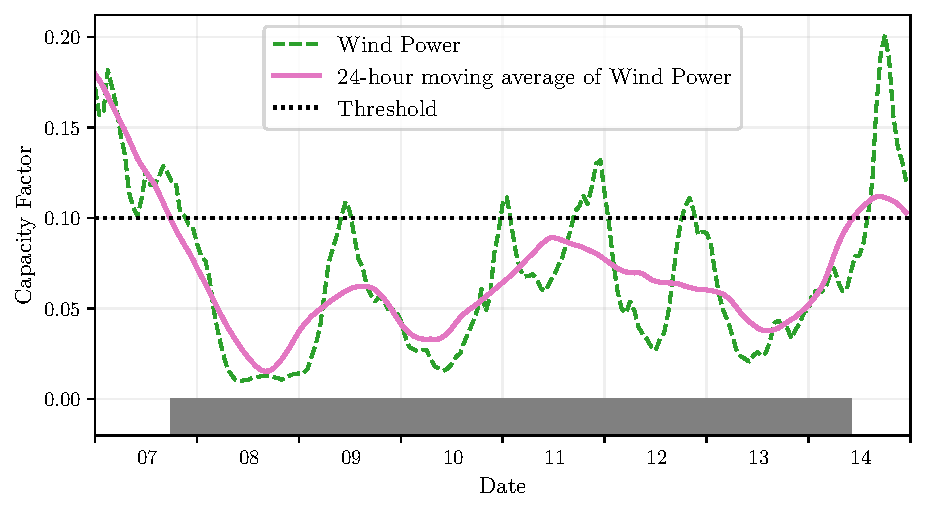
\includegraphics[width=\textwidth]{droughts_methodology.pdf}
	\caption{Wind time series of CF (green) and its 24-hour moving average (pink) from the 7th to the 15th of July 2021. The black dashed line indicates the CF threshold. The grey bar shows the period identified as a wind drought under our definition}
	\label{fig:find_res_droughts}
\end{figure}

The moving average approach smooths out short-term fluctuations, so that brief periods above the threshold do not interrupt an otherwise continuous low-CF period (Fig.~\ref{fig:find_res_droughts}). This means that a single hour above the threshold does not "break" a RES drought event if it is surrounded by prolonged low-generation hours. As a result, fewer but longer-lasting RES drought events are identified, which may better reflect real-world conditions where energy supply constraints persist over extended periods.

\section{Results}
\label{sec:results}

\subsection{Verification}
\label{sec:verification}

The accuracy of the datasets used in this study was verified, before continuing to the analysis of RES droughts. For the verification process, time-varying values of installed capacity were used to account for changes in RES development over the verification period. This step allowed us to assess how well the datasets represent the production of renewable energy by comparing them against observed data. The general statistics of the observed data and the three datasets are presented in the violin plots in Fig.~\ref{fig:violin_plots}, considering the 2014-2023 validation period for wind and 2023 for solar PV. These plots illustrate the density of CF values for each dataset, highlighting differences between the datasets and their alignment with observed data. The general CF values show ATL aligns better with OBS for wind, and all datasets are similar for PV.

\begin{figure}[ht!]
	\centering
	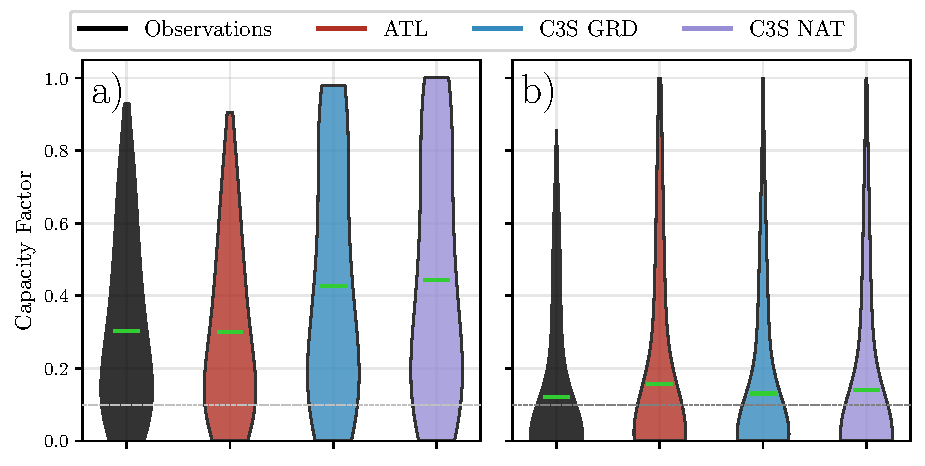
\includegraphics[width=\textwidth]{violin_plots_verification.pdf}
	\caption{Violin plots of CF distributions for wind a) and solar PV b) datasets. Each violin represents the distribution of CF over time for different datasets: Observations (black), ATL (red), C3S GRD (blue), and C3S NAT (purple). The mean value for each dataset is marked with a green horizontal line. The red line indicates the threshold of 0.1 used in the study to identify RES droughts}
	\label{fig:violin_plots}
\end{figure}

\subsubsection{Wind Energy}
\label{sec:wind_verification}

The C3S datasets use the Vestas V136/3450 wind turbine power curve (Fig.~\ref{fig:power_curve}a). The Atlite model allows the user to specify the power curve. We considered the 121 power curves available for download from Renewables.ninja~\citep{staffell2016wake}. For each power curve, Renewables.ninja also provides four associated smoothed power curves. The smoothing is done using a Gaussian filter with different standard deviations that depend on the wind speed. A separate wind CF time series for Ireland was generated for each of the wind turbine power curves and smoothing levels.

The performance of each CF time series is then assessed based on four skill scores: correlation coefficient (CC), root mean square error (RMSE), mean bias error (MBE), and the percentage of overlap. The percentage of overlap quantifies the similarity between the observed and modelled distributions. It is a positively oriented skill score, where 100\% shows full agreement between the two distributions, and 0\% indicates no overlap. The histograms of hourly CF values for the most recent decade (2014-2023) are used to calculate this skill score.

\begin{figure}[!ht]
	\centering
	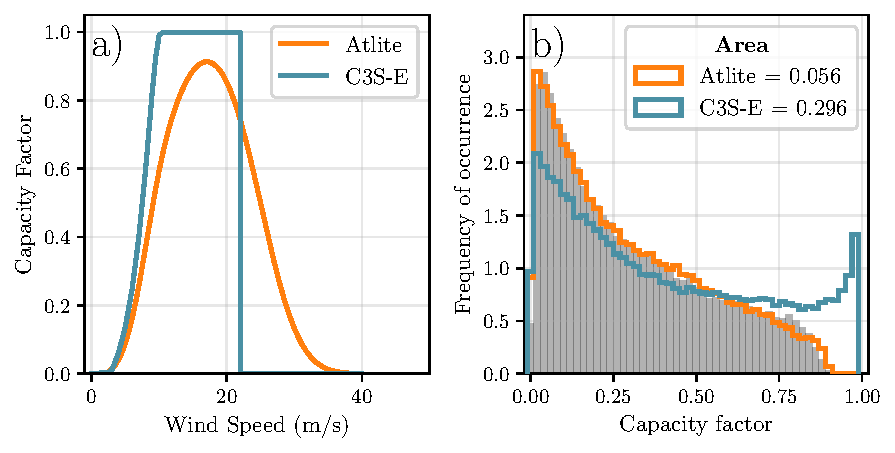
\includegraphics[width=\textwidth]{verification_power_curve.pdf}
	\caption{a) Power curves of the Enercon E112.4500 with a 0.3w smoothing filter used by ATL (orange) and the Vestas V136/3450 used by C3SE (blue) b) Histograms of wind CF for Ireland from ATL (orange), C3SE (blue) and Observed (shaded)}
	\label{fig:power_curve}
\end{figure}

Based on these metrics, the most representative power curve for Ireland is the Enercon E112.4500 power curve with the $0.3w$ smoothing filter. The smoothing of the wind turbine power curve represents losses associated with each turbine, as well as losses such as wake effects between turbines, which are important when modelling wind energy on larger spatial scales. The histogram in Fig.~\ref{fig:power_curve}b shows that the C3SE power curve tends to underestimate low CF values and overestimate higher ones, whereas the smoothed ATL power curve more closely follows the observed wind availability data. This is further supported by the percentage of overlap which is higher for ATL (97.2\%) than for C3SE (83.2\%), indicating better agreement with observed data.

\begin{figure}[!ht]
	\centering
	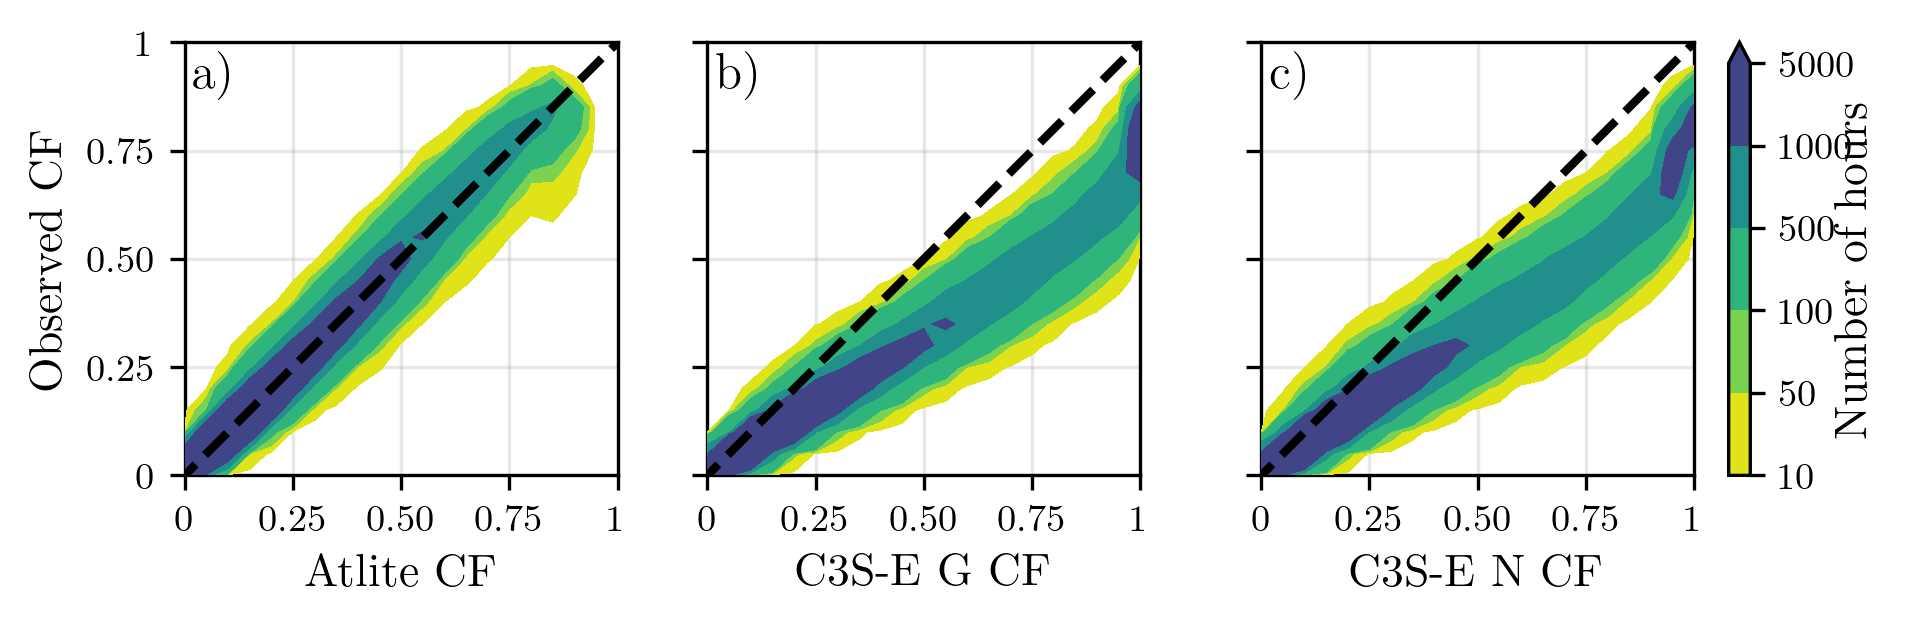
\includegraphics[width=\textwidth]{verification_wind_contour.png}
	\caption{Wind CF density plot of the observed CF (vertical axes) and modelled (horizontal axes) CF data for the a) ATL, b) C3S GRD and c) C3S NAT datasets}
	\label{fig:wind_verification_contour}
\end{figure}

The effect of the difference between the power curves is also visible in Fig.~\ref{fig:wind_verification_contour}, which shows a density plot of wind CF values. The two C3S datasets are shown to overestimate the observed CF, whereas the ATL dataset is in good agreement with the observed data. The skill scores presented in Table~\ref{tab:wind_skill_scores} show that ATL performs better than the two C3S datasets for all of the skill scores. 

\begin{table}[!ht]
	\centering
	\begin{tabular}{l|lll|}
		\cline{2-4}
		& \textbf{ATL} & \textbf{C3S GRD} & \textbf{C3S NAT} \\ \hline
		\multicolumn{1}{|l|}{\textbf{CC}}   & 0.981           & 0.972            & 0.970            \\ \hline
		\multicolumn{1}{|l|}{\textbf{RMSE}} & 0.045           & 0.177            & 0.162            \\ \hline
		\multicolumn{1}{|l|}{\textbf{MBE}}   & -0.003          & 0.137            & 0.121            \\ \hline
	\end{tabular}
	\caption{Skill scores for wind power for the three datasets compared to observed data}
	\label{tab:wind_skill_scores}
\end{table}

Fig.~\ref{fig:bar_number_events_verification_wind} shows the average annual number of wind drought events during the 2014 to 2023 validation period. The figure reveals that ATL presents the best overall agreement with the observed frequency and duration of wind drought events. This pattern is particularly evident for shorter-duration events, which are the most frequent.

\begin{figure}[!ht]
	\centering
	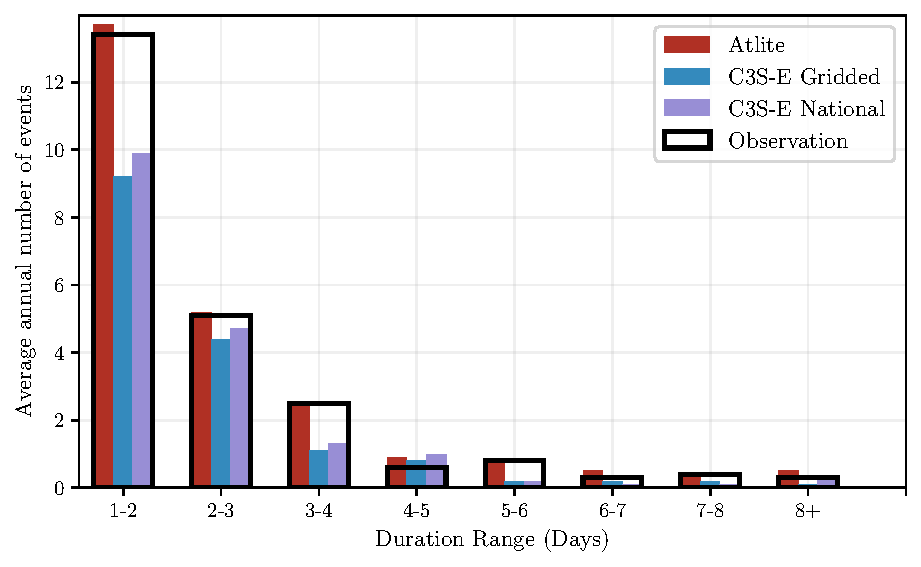
\includegraphics[width=\textwidth]{verification_wind_number_events.pdf}
	\caption{Average annual number of wind drought events for ATL (red), C3S GRD (blue), C3S NAT (purple), and the observed data (black outline). The wind droughts are identified from 2014 to 2023, considering the actual capacity of the system at any given time}
	\label{fig:bar_number_events_verification_wind}
\end{figure}

This verification for wind generation data highlights the importance of selecting a representative wind turbine power curve for the region being analysed. The ATL dataset, which uses a representative wind turbine power curve, is skilled at reproducing wind CF and RES droughts over Ireland. On the other hand, the power curve used for both C3S GRD and C3S NAT is not representative for Ireland, as it severely overestimates generation, underestimating the occurrence of RES droughts. This highlights a problem with using generalised datasets for analysing RES droughts: biases severely affect their ability to accurately reproduce RES drought events. The skill scores for the three datasets (Tab.~\ref{tab:wind_skill_scores}) show only a small difference in their ability to reproduce the changes in CF, as seen by their similar CC scores. However, their ability to reproduce the actual CF values is much lower than that of ATL, with RMSE scores almost four times bigger for the two C3S datasets. There is a clear bias towards an overestimation of CF, seen in the MBE values, which leads to the underestimation of RES droughts. This highlights the need to use regionally verified models to assess RES droughts.

\subsubsection{Solar PV Energy}
\label{sec:pv_verification}

The Atlite model allows the user to select certain PV panel characteristics. In this study, the three PV panel types available in the Atlite model were considered (CSi, CdTe, Kaneka). Following the same methodology as in the previous section, the three available models were compared using four skill scores (CC, RMSE, MBE, and the percentage of overlap). Based on the best-performing metrics, the Beyer PV panel model was selected~\citep{beyer2004pv}, using the Kaneka Hybrid panel option. For all solar PV farm locations, the azimuth angle is fixed at 180\textdegree (due south), and the optimal tilt angle option is applied. 

The solar PV installed capacity available on the spreadsheets from EirGrid represents the Maximum Export Capacity (MEC) and does not accurately reflect the installed solar PV capacity. To enable actual solar PV generation potential to be modelled correctly, installed capacities were set at 1.4 times the MEC values. This scaling factor was estimated by analysing proprietary data from individual solar PV farms provided by EirGrid, which showed that, on average, assuming that the installed capacities of farms exceed their MEC values by 40\% yields the best agreement with the observed availability.

\begin{figure}[h!]
	\centering
	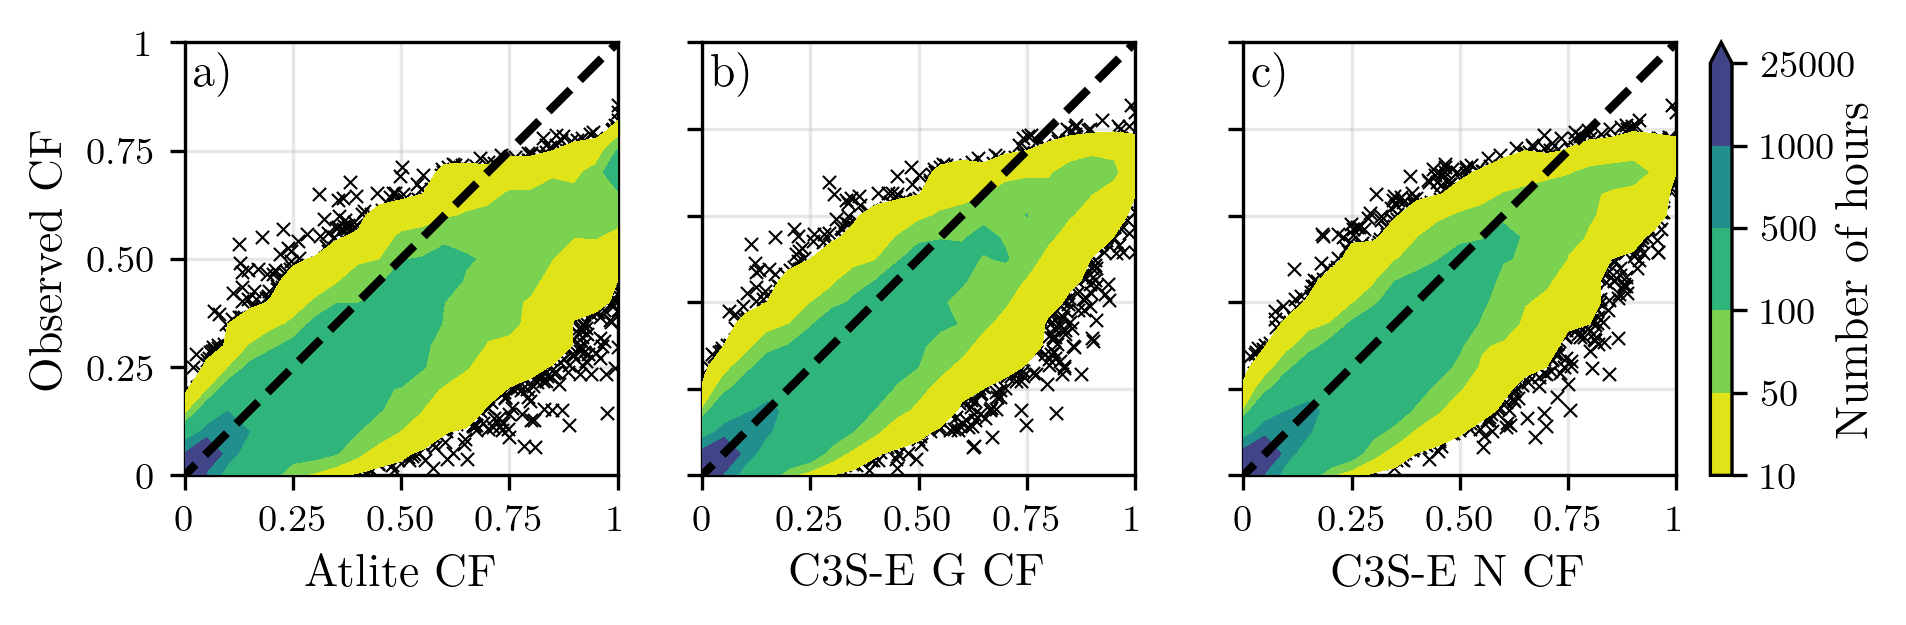
\includegraphics[width=\textwidth]{verification_pv_contour.png}
	\caption{Solar PV CF density plot of the observed (vertical axes) and modelled (horizontal axes) CF series for the a) ATL, b) C3S GRD and c) C3S NAT datasets}	
	\label{fig:solar_verification_contour}
\end{figure}

Fig.~\ref{fig:solar_verification_contour} shows that the three datasets have a similar tendency to overestimate the CF compared to the observed values, especially for high CF values. The skill scores presented in Table~\ref{tab:pv_skill_scores} indicate that C3S GRD and C3S NAT perform better than ATL for solar PV CF, with lower RMSE and MBE, and higher CC scores. This may be due to the statistical approach taken by C3SE for the orientation of the PV panels.

\begin{table}[!ht]
	\centering
	\begin{tabular}{l|lll|}
		\cline{2-4}
		& \textbf{ATL} & \textbf{C3S GRD} & \textbf{C3S NAT} \\ \hline
		\multicolumn{1}{|l|}{\textbf{CC}}   & 0.921           & 0.931            & 0.931            \\ \hline
		\multicolumn{1}{|l|}{\textbf{RMSE}} & 0.119           & 0.090            & 0.113            \\ \hline
		\multicolumn{1}{|l|}{\textbf{MBE}}   & 0.046           & 0.027           & 0.021           \\ \hline
	\end{tabular}
	\caption{Skill scores for solar PV CF for the three datasets compared to observed data}
	\label{tab:pv_skill_scores}
\end{table}

Fig.~\ref{fig:bar_number_events_verification_pv} shows the number of solar PV drought events during the 2023 validation period across different duration ranges. The figure reveals partial agreement between the three datasets and the observed data, with consistent results noticed for duration ranges of 1-2, 3-4, 7-8, and 8+ days. However, discrepancies appear in the other ranges, where the models diverge from the observed data. The main challenge in validating solar PV data stems from the recent installation of a large share of Ireland’s solar PV capacity, with over 65\% of the total solar PV capacity installed in 2023. This results in uncertainties in solar PV generation data and the actual generating capacity in the first few months after each farm is connected. Overall, C3S GRD performs slightly better than the other datasets in reproducing observed solar PV drought events.

\begin{figure}[!ht]
	\centering
	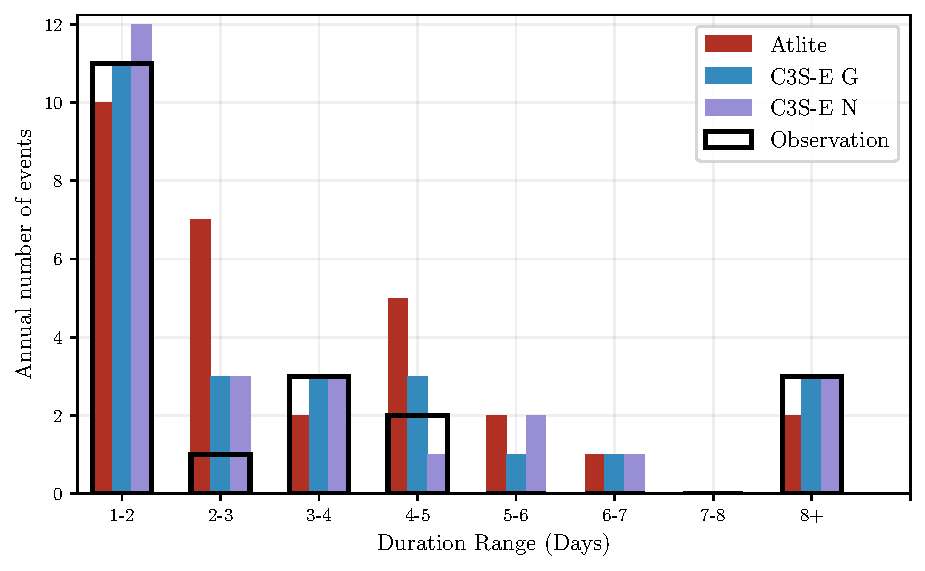
\includegraphics[width=\textwidth]{verification_pv_number_events.pdf}
	\caption{Number of solar PV drought events for ATL (red), C3S GRD (blue), and C3S NAT (purple) and the observed data (black outline). The solar PV droughts are identified for 2023, considering the actual capacity of the system at any given time}
	\label{fig:bar_number_events_verification_pv}
\end{figure}

\subsection{Analysis}
\label{sec:analysis}

In this section, RES droughts are analysed by calculating the frequency and duration of RES drought events, the return periods for different RES drought durations, and the seasonality of RES drought events. Understanding the characteristics and timing of RES drought events enables system operators to optimally plan for reserve capacity requirements, ensuring grid stability and security of supply. Results are presented for the three datasets, allowing their differences on the characterisation of RES droughts to be clearly identified.

RES drought events are evaluated under two different scenarios with fixed installed capacities: the 91W-9PV scenario, with 5.9 GW of wind capacity and 0.6 GW of solar PV capacity; and the 57W-43PV scenario, where wind capacity comprises 11.45 GW and solar PV capacity increases to 8.6 GW. Both scenarios were driven by 45 years of ERA5 data. Using the RES drought identification process described in Section~\ref{sec:res_drought}, wind and solar PV droughts are first analysed separately before presenting the results for combined (wind + solar PV) RES droughts under both scenarios.

\subsubsection{Annual Number of RES Droughts}

The first part of the analysis examines the annual number of RES drought events. When only wind energy is considered (Fig.~\ref{fig:boxplot_number_events}a), the number of RES drought events decreases as the duration range increases, with very few events lasting more than seven days. In contrast, for solar PV energy (Fig.~\ref{fig:boxplot_number_events}b), RES drought frequency declines from one to eight days and then slightly increases for longer durations. This behaviour is attributable to Ireland's high-latitude location, where reduced sunlight in winter (from November to March) leads to consistently low solar PV output.

Moreover, the comparison between wind and solar PV results indicates that the median, first, and third quartiles for solar PV are consistently higher than or equal to those for wind. This is expected, given that solar PV generation is inherently lower, zero at night, and limited by the solar cycle. When wind and solar PV are combined under the 91W-9PV scenario (Fig.~\ref{fig:boxplot_number_events}c), the results closely mirror those of wind alone, due to the dominance of wind power in the current energy mix. However, in the 57W-43PV scenario (Fig.~\ref{fig:boxplot_number_events}d), a marked reduction in RES drought events is observed across all datasets, with a decrease of the total number of events of 56\% for ATL, 52\% for C3S GRD, and 50\% for C3S NAT, demonstrating the beneficial effects of a more balanced energy mix.

The consistently higher RES drought counts reported by the ATL dataset, compared to the C3S datasets, underscore the importance of wind turbine power curve representation when quantifying RES droughts. Whereas the three datasets agree on the overall effect of balancing the share of wind and solar PV generation, they differ at a quantitative level, which has crucial implications for energy planning.

\begin{figure}[!ht]
	\centering
	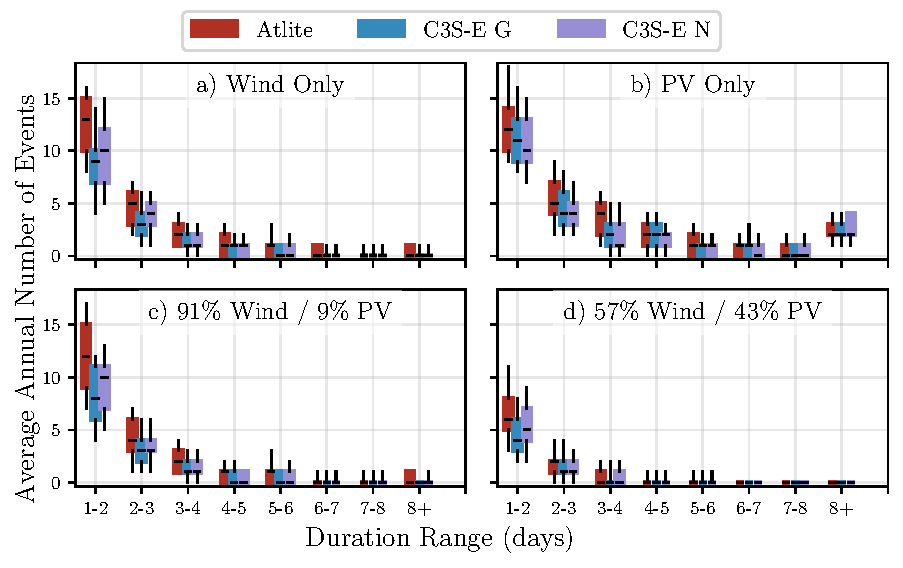
\includegraphics[width=\textwidth]{droughts_number_events.pdf}
	\caption{Average annual number of RES droughts (from 1979 to 2023) for a)~Wind, b)~solar PV, c)~91W-9PV and d)~57W-43PV for ATL (red), C3S GRD (blue), and C3S NAT (purple). The x-axis represents duration ranges in days (lower bound included), while the y-axis indicates the annual number of events. The boxes display the first and third quartiles and the median is marked by a black line. The whiskers indicate the 5th and 95th percentiles}
	\label{fig:boxplot_number_events}	
\end{figure}

\subsubsection{Return Periods of RES Drought Duration}

RES drought events identified over the 45-year period were used to calculate the return periods for different RES drought durations. A return period is the estimated average time interval between events of a specified duration (not to be confused with the frequency of their occurrence within a fixed time frame). Fig.~\ref{fig:return_periods} shows the return periods for different RES drought durations, which can be used to capture the most extreme events affecting the system. Understanding their return periods is crucial, as extreme yet rare RES droughts pose the toughest challenge to energy security by placing significant strain on the conventional backup sources necessary to maintain security of supply during these events.

The duration of wind droughts (Fig.~\ref{fig:return_periods}a) increases in a log-linear fashion across the three datasets. The log-linear trend indicates a predictable relationship between wind drought duration and occurrence, with longer wind droughts becoming exponentially less likely as duration increases. In the case of solar PV droughts (Fig.~\ref{fig:return_periods}b), Atlite behaves differently than the two C3S datasets. The ATL dataset show a generally log-linear increase. For C3S GRD and C3S NAT, the duration of PV droughts increases in a log-linear pattern for events lasting less than 16 days. Beyond this duration, there is a sharp rise in solar PV drought duration for events up to a one-year return period. This sudden increase again reflects the impact of extended periods of low PV generation during winter in Ireland. The difference between the ATL and the C3S results arises from differences in the datasets near the threshold of 0.1 CF. ATL remains slightly above the threshold more frequently during these conditions, leading to shorter, more fragmented RES drought events. In contrast, C3S GRD and C3S NAT tend to fall below the threshold in similar conditions, resulting in longer continuous RES drought periods, especially during winter.

Under the 91W-9PV scenario (Fig.~\ref{fig:return_periods}c), the combined RES drought return periods mirror those for wind alone, reflecting the dominance of wind in the current energy mix. In contrast, the 57W-43PV scenario (Fig.~\ref{fig:return_periods}d) shows a dramatic increase in return periods across all durations, suggesting that a more diversified energy mix can substantially mitigate the frequency of prolonged RES drought events. For example, the return period for a five-day RES drought event (shown by the vertical dashed lines in Fig.~\ref{fig:return_periods}) extends from roughly six months for the 91W-9PV scenario, to four years for the 57W-43PV scenario in the ATL dataset, and from about fifteen months to around five years in the two C3S datasets. Despite the lower wind share in the 57W-43PV scenario, typically known for its relative stability, the balanced share with solar PV leads to extended return periods for RES droughts. This result indicates that the complementarity between wind and solar PV plays a crucial role in reducing the occurrence of RES drought events in a diversified energy portfolio.

\begin{figure}[!ht]
	\centering
	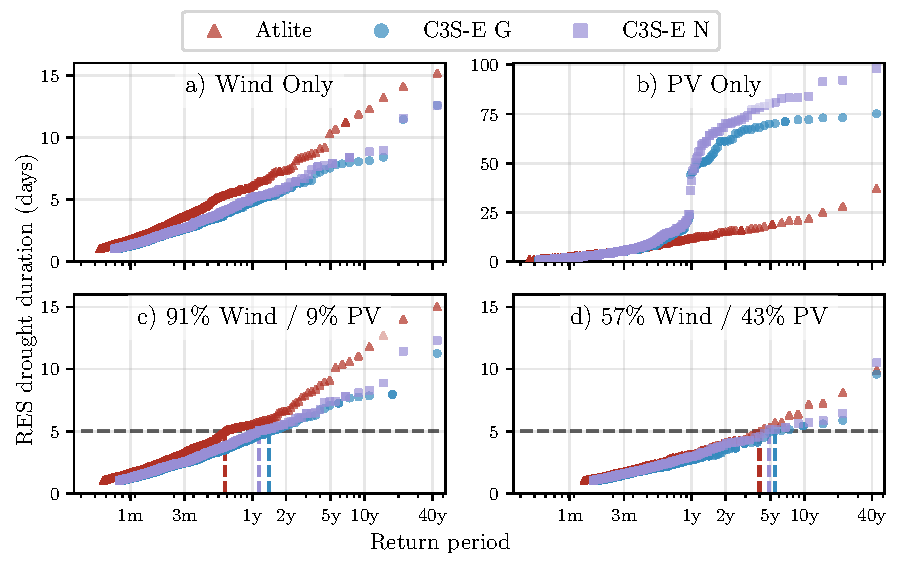
\includegraphics[width=\textwidth]{droughts_return_periods.pdf}
	\caption{Return periods of the duration of RES droughts  (from 1979 to 2023) for a)~Wind, b)~Solar PV, c)~91W-9PV and d)~57W-43PV for ATL (red triangle), C3S GRD (blue circle), and C3S NAT (purple square). The x-axis represents the return period time in a log-scale and the y-axis indicates the duration of RES drought associated with it. The horizontal dashed line marks the 5-day return period, with coloured vertical dashed marking its return period for each dataset}
	\label{fig:return_periods}
\end{figure}

Across Fig.~\ref{fig:return_periods}a, c, and, d, the return periods in the ATL dataset are consistently higher than those in the two C3S datasets. For instance, in the 91W-9PV scenario (Fig.~\ref{fig:return_periods}c), an event with a one-year return period lasts six days in the ATL dataset, compared to only five days in the C3S datasets. This difference underscores the importance of model selection when quantifying RES droughts, as each dataset’s assumptions and parametrisations significantly influence RES droughts duration estimates. Additionally, in all four graphs, the similarity between results from the two C3S datasets suggests that assumptions in the ATL dataset, such as wind turbine power curve selection and PV panel specifications, have a greater impact on RES drought duration estimates than the precise geographic distribution of RES farms when studying the return periods of RES droughts.

The return periods calculated from the three datasets show large differences, in particular for the more extreme events with longer return periods. The C3S datasets produce shorter RES drought durations for these events, which would have the largest impact on the power system. This shows that system planning based on the wrong datasets could yield an underestimation of the duration of extreme RES droughts, potentially leading to shortages linked to undersized reserve capacity.

\subsubsection{Seasonal Distribution of RES Droughts}

The seasonal analysis of RES droughts is based on the percentage of hours in each month classified as part of a RES drought event. Wind droughts tend to be more frequent during summer, whereas solar PV droughts are more common in winter due to reduced sunlight. By comparing these seasonal patterns across different datasets and energy scenarios, this study examines how model-specific assumptions and variations in capacity mix affect the overall characterisation of RES drought events.

For the wind-only scenario (Fig.~\ref{fig:res_droughts_seasonality}a), the ATL dataset exhibits a pronounced seasonal pattern, with about 24\% of summer hours (June, July, August) identified as RES droughts compared to only 4\% in winter (December, January, February). This strong seasonal signal is less evident in the C3S datasets, which suggests that the differences in the underlying wind power curves play a significant role. In ATL, CF near or below the 0.1 threshold occurs at relatively higher wind speeds, resulting in a higher count of RES drought hours during the summer months. In contrast, solar PV droughts (Fig.~\ref{fig:res_droughts_seasonality}b) display an opposite seasonal trend. Across all datasets, over 60\% of winter hours are classified as solar PV droughts, reflecting the naturally low solar irradiance in Ireland during winter. 

ATL tends to record a slightly higher percentage of RES drought hours for wind and a marginally lower percentage for solar PV relative to the C3S datasets. These differences highlight how dataset-specific assumptions, such as the treatment of wind turbine power curves and PV panel characteristics, significantly influences the apparent seasonal dynamics of RES droughts.

The 91W-9PV scenario (Fig.~\ref{fig:res_droughts_seasonality}c) shows patterns comparable to the ones for wind droughts (Fig.~\ref{fig:res_droughts_seasonality}a). However, in the 91W/9PV scenario, the number of hours classified as RES droughts in summer decreases slightly compared to the wind-only scenario. This reduction can be explained by the contribution of solar PV generation during the summer months in the 91W-9PV scenario, even though it constitutes only 11\% of total capacity. Since the number of RES drought hours for solar PV in summer is near zero, this small contribution has a noticeable impact on reducing overall RES drought hours. In the 57W-43PV scenario (Fig.~\ref{fig:res_droughts_seasonality}d), all three datasets show a reduction in monthly RES drought frequency. Annual reductions in median RES drought frequency are observed across the datasets, dropping from 14\% to 5\% for ATL, from 8\% to 3\% for C3S GRD, and from 9\% to 4\% for C3S NAT. The balanced mix of wind and solar PV power in this scenario reduces the seasonal signal overall and significantly decreases the percentage of RES drought hours in the summer.

\begin{figure}[!ht]
	\centering
	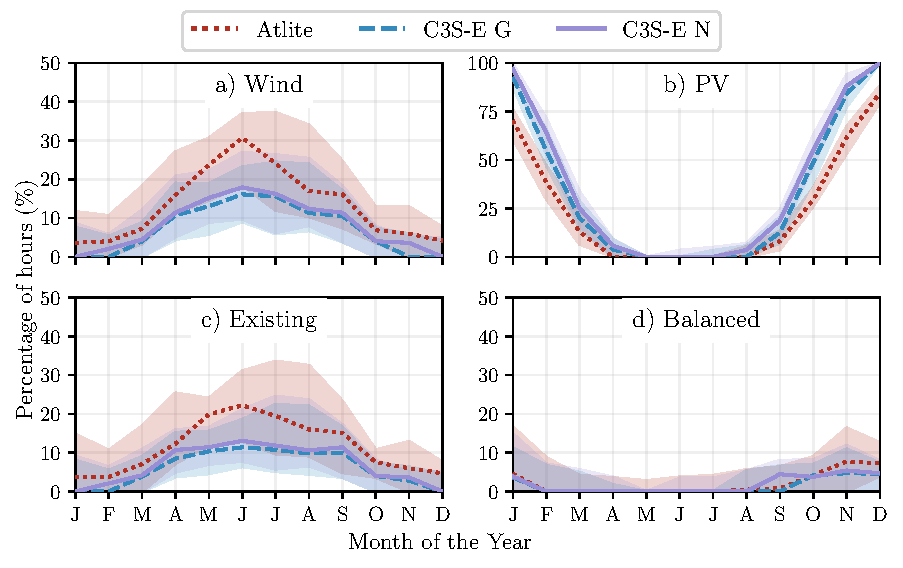
\includegraphics[width=\textwidth]{droughts_seasonality.pdf}
	\caption{Percentage of hours in a month which are part of a RES drought (from 1979 to 2023) for a)~Wind, b)~Solar PV, c)~91W-9PV and d)~57W-43PV for ATL (red dotted), C3S GRD (blue dashed), and C3S NAT (purple solid). The x-axis represents the month of the year, and the y-axis indicates the percentage of hours. Lines correspond to the median values and the area between the first and third quartiles is shaded. Note the different y-axis scale for b).}
	\label{fig:res_droughts_seasonality}
\end{figure}

The seasonal variations of RES droughts observed in this study have important implications for energy planning. Energy demand peaks in winter for Northern European countries, making the seasonality of RES droughts critical for the sizing of reserve capacity. Our results show that selecting the wrong dataset could severely underestimate RES droughts during winter months, thereby affecting the reliability of the energy system during critical periods. Additionally, the integration of large shares of solar PV in the system leads to a generalised reduction of RES droughts, yet winter months present a slight increase. The natural limitations of solar PV lead to inevitably higher reserve capacity needs during winter months as reliance on RES increases. These types of insights are essential to develop targeted strategies that enhance grid resilience and ensure a stable energy supply throughout the year.


\section{Conclusions}
\label{sec:conclusions}

The two questions presented and answered in this study are: XXX?; YYY? Three different datasets were compared over a 45-year period: one created using a regionally validated model and two derived from a generic dataset for Europe, C3S-Energy. The two datasets derived from C3S-Energy present different approaches, with one using large-scale aggregated information only, and the other one including the locations of farms as well. The regionally validated model considered the locations of farms as well as tailored wind and solar PV models selected to best represent the actual generation in Ireland.

% Answer XXX - generic models are sufficient to quantify RES droughts
Our results show the limitations in the quantification of RES droughts present in datasets that have not undergone regional validation. The three datasets used in this study are able to capture overall trends in RES drought occurrence such as the seasonal cycle or the effect of increasing the share of solar PV. However, significant differences in the quantitative values, particularly the extremes, emerge when using non-validated datasets for the study of RES droughts. This finding highlights that using a non-validated dataset can lead to undersized reserve capacity, with the associated negative consequences for grid stability and security of supply.

This study has also revealed that differences in the wind turbine power curves and solar PV panel models have a stronger influence on the estimation of RES droughts than the consideration of RES farm locations. The two datasets derived from C3S-Energy consistently underestimated the number of wind drought events and the frequency of extremes when compared to the regionally validated dataset with a specifically selected wind turbine power curve. This suggests that a meticulous selection of the wind turbine power curve to match observed data is crucial for accurately quantifying RES drought risks, thereby supporting more effective energy system planning.

% Answer YYY - role of intergrating PV
Finally, the effect of the integration of solar PV in a wind-dominated system on RES droughts has been explored in a real-case setting based on Ireland. Our analysis has demonstrated that transitioning to a system with similar amounts of wind and solar PV reduces the frequency, duration, and seasonal variability of RES drought events. This improvement is attributed to the complementary nature of wind and solar PV generation, as solar PV typically peaks in summer while wind generation is more consistent in winter. However, this integration is unable to counter the critical winter RES droughts, which coincide with the strongest electricity demand in Northern European countries like Ireland. Still, a more diversified renewable energy mix mitigates extreme RES drought conditions and enhances overall system resilience.

% Limitations
The results presented in this study have four main limitations. First, the presented study uses a fixed threshold to define RES drought events, but other methods could yield different results, even though the main takeaways would be expected to be the same. Second, the definition of RES droughts based on generation does not consider the important role of demand, which could be of interest to system operators. Third, the availability of solar PV data is limited to a relatively short time period, as recent expansions in installed capacity have significantly changed the generation landscape. Lastly, the source for weather data is ERA5, which is among the best reanalysis datasets for renewable energy applications, but still comes in a limited spatial resolution, an issue that can be addressed once higher resolution datasets become available. 

% Future work
Future work is planned to extend the current analysis. First, climate projection data will be integrated with different energy scenarios, incorporating the addition of offshore wind, to better understand how climate change might affect RES droughts. Second, expanding the geographic domain of the study to include the rest of Europe would provide a more comprehensive understanding of RES droughts in an interconnected electricity grid. This would require extensive verification across other European countries, making it a more complex but highly relevant challenge.

\section*{Data Availability}

The ERA5 data can be obtained from the Climate Data Store (\url{https://doi.org/10.24381/cds.adbb2d47}). The C3SE dataset is also available from the Climate Data Store (\url{https://doi.org/10.24381/cds.4bd77450}). Information on wind and solar PV farms in Ireland can be obtained from the EirGrid website (\url{https://www.eirgrid.ie/grid/system-and-renewable-data-reports}). The Atlite model used in this study is open-source and can be found on GitHub (\url{https://github.com/pypsa/atlite}). The data and code required to reproduce the analysis in this article will be made available upon acceptance of the manuscript in a public GitHub repository.

\section*{Acknowledgments}

The research conducted in this publication was funded by Science Foundation Ireland and co-funding partners under grant number 21/SPP/3756 through the NexSys Strategic Partnership Programme.

\bibliographystyle{elsarticle-num-names}
\bibliography{RES_droughts_Morin_ref}

\end{document}

\endinput



